%
%
%% Enter Figures and Tables here:
%
% DO NOT USE \psfrag or \subfigure commands.
%
% Figure captions go below the figure.
% Table titles go above tables; all other caption information
%  should be placed in footnotes below the table.
%
%----------------
% BEGIN FIGUREs
%

\clearpage
\begin{figure}[t]
  \begin{center}
    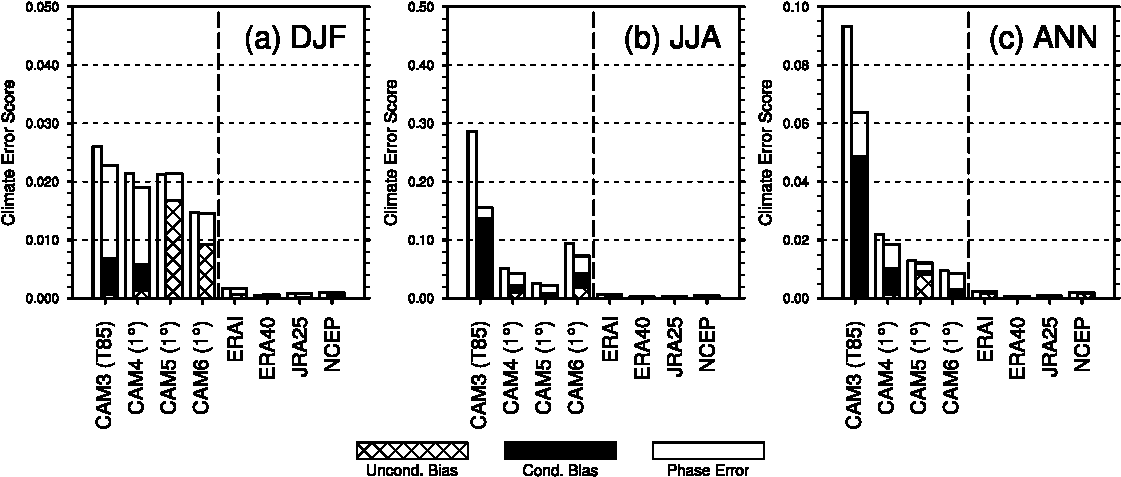
\includegraphics[width=1\textwidth,angle=0.]{./figs/f_skill_score.pdf}
 \end{center}
  \caption {Seasonal climatology of contributions to the Normalized Mean Square Error (NMSE) over the northern hemisphere (30$^\circ$ N-90$^\circ$ N) for CAM releases between CAM3 and CAM6. Individual contributions are the unconditional bias (hatched), conditional bias (solid) and phase error (unfilled). The narrow unfilled bar for each model is the scaled variance ratio (SVR). The model is compared to the ECMWF (ERA15) reanalysis. Contemporary analysis (JRA25/NCEP/ERA40 and ERA-interim) biases compared top ECMWF are also shown.} 
\label{f_skill_score}
\end{figure} 
%%
\clearpage
\begin{figure}[t]
  \begin{center}
    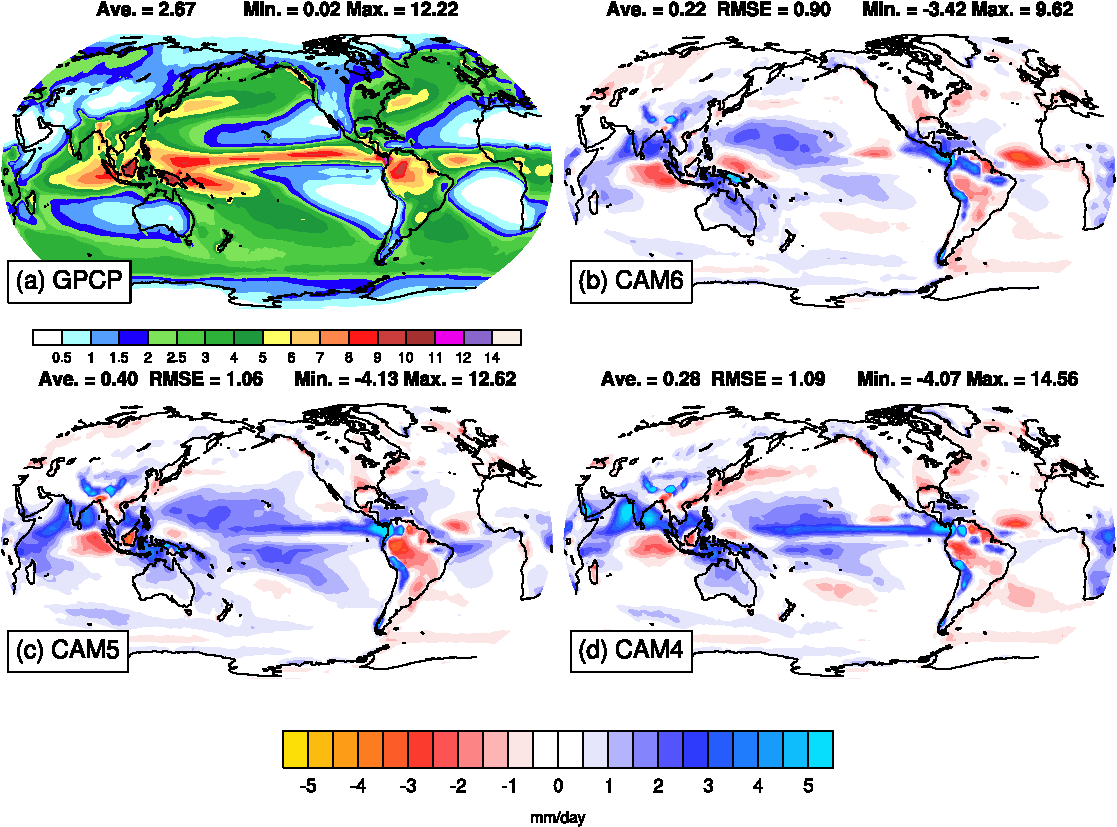
\includegraphics[width=1.\textwidth,angle=0.]{./figs/f_PRECT_2D_CAM456.pdf}
  \end{center}
  \caption{Climatology of annual precipitation (mm/day) for (a) Observations (GPCP, 19XX-20XX), and its biases for (a) CAM4 (b) CAM5  through CAM6 AMIP simulations for the period 1979-2005} 
\label{f_PRECT_2D_CAM456}
\end{figure} 
%%
\clearpage
\begin{figure}[t]
  \begin{center}
    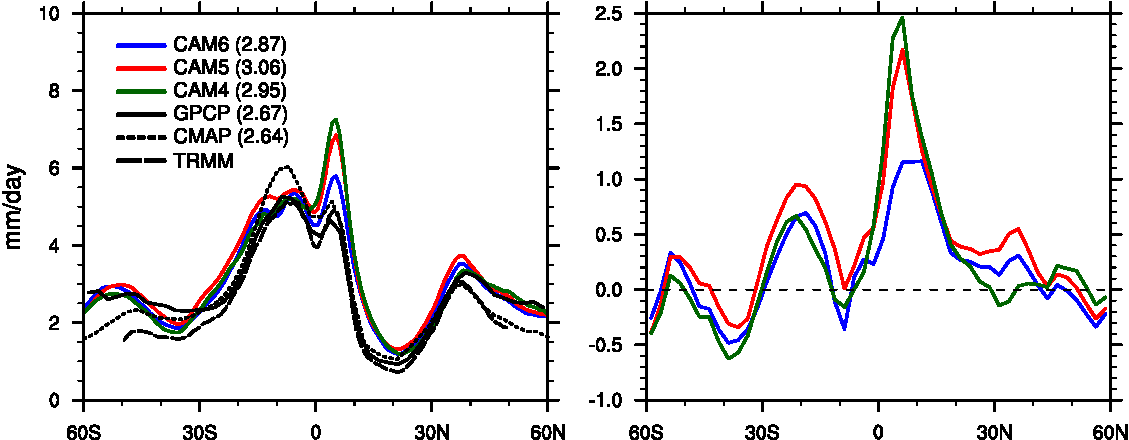
\includegraphics[width=1.\textwidth,angle=0.]{./figs/f_PRECT_1D_DJF_CAM456.pdf}
  \end{center}
  \caption{Climatology of annual precipitation (mm/day) for (a) Observations (GPCP, 19XX-20XX), and its biases for (a) CAM4 (b) CAM5  through CAM6 AMIP simulations for the period 1979-2005} 
\label{f_PRECT_1D_DJF_CAM456}
\end{figure} 
%%
\clearpage
\begin{figure}[t]
  \begin{center}
    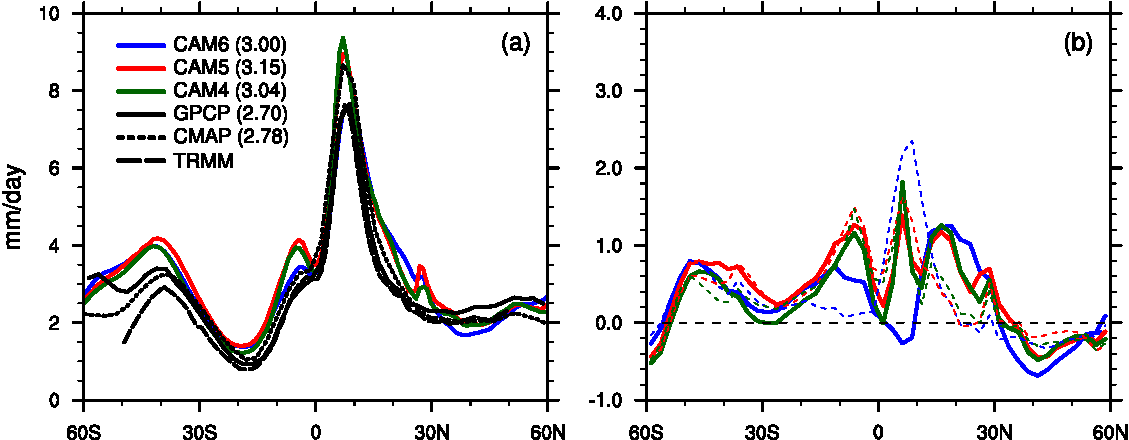
\includegraphics[width=1.\textwidth,angle=0.]{./figs/f_PRECT_1D_JJA_CAM456.pdf}
  \end{center}
  \caption{Climatology of annual precipitation (mm/day) for (a) Observations (GPCP, 19XX-20XX), and its biases for (a) CAM4 (b) CAM5  through CAM6 AMIP simulations for the period 1979-2005} 
\label{f_PRECT_1D_JJA_CAM456}
\end{figure} 

%%
\clearpage
\begin{figure}[t]
  \begin{center}
    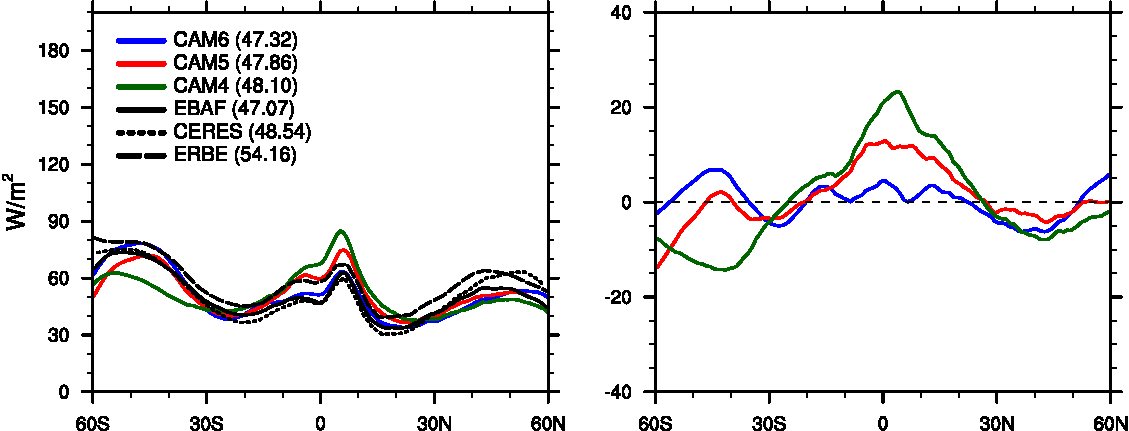
\includegraphics[width=1.\textwidth,angle=0.]{./figs/f_SWCF_1D_ANN_CAM456.pdf}
  \end{center}
  \caption{Climatology of annual precipitation (mm/day) for (a) Observations (GPCP, 19XX-20XX), and its biases for (a) CAM4 (b) CAM5  through CAM6 AMIP simulations for the period 1979-2005} 
\label{f_SWCF_1D_ANN_CAM456}
\end{figure} 

%%
\clearpage
\begin{figure}[t]
  \begin{center}
    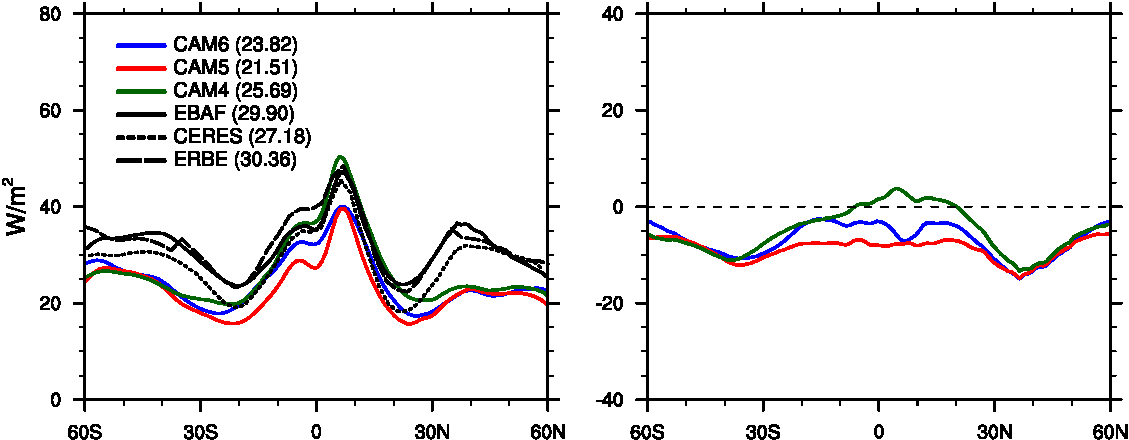
\includegraphics[width=1.\textwidth,angle=0.]{./figs/f_LWCF_1D_ANN_CAM456.pdf}
  \end{center}
  \caption{Climatology of annual precipitation (mm/day) for (a) Observations (GPCP, 19XX-20XX), and its biases for (a) CAM4 (b) CAM5  through CAM6 AMIP simulations for the period 1979-2005} 
\label{f_LWCF_1D_ANN_CAM456}
\end{figure} 

%%
\clearpage
\begin{figure}[t]
  \begin{center}
    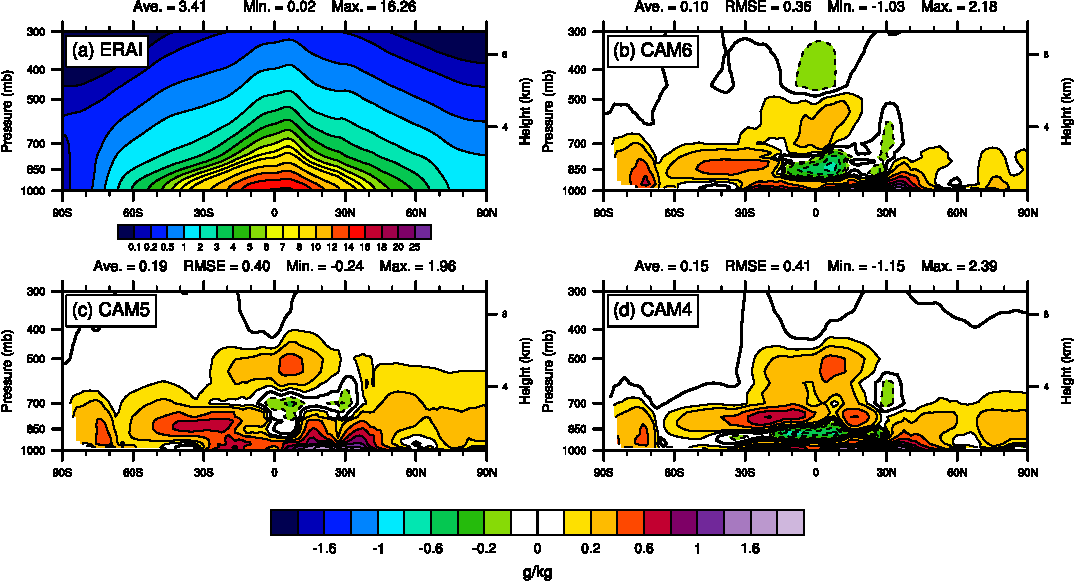
\includegraphics[width=1.\textwidth,angle=0.]{./figs/f_MERRA_Q_latp_diff_ANN.pdf}
  \end{center}
  \caption{Climatology of annual precipitation (mm/day) for (a) Observations (GPCP, 19XX-20XX), and its biases for (a) CAM4 (b) CAM5  through CAM6 AMIP simulations for the period 1979-2005} 
\label{MERRA_Q_latp_diff_ANN}
\end{figure} 